%======================================================
% This file is part of
% "AMCOS_booklet"
% Version 1.1 (04/07/2019)
% A LaTeX template for conference books of abstracts
%
% This template is available at:
% https://github.com/maximelucas/AMCOS_booklet
%
% License: GNU General Public License v3.0
%
% Authors:
% Maxime Lucas (ml.maximelucas@gmail.com)
% Pau Clusella
%=======================================================

\documentclass[openany, parskip=full, 12pt, a4]{scrbook}

% For tables
\usepackage{booktabs}

\input{preamble}
%======================================================
% This file is part of
% "AMCOS_booklet"
% Version 1.1 (04/07/2019)
% A LaTeX template for conference books of abstracts
%
% This template is available at:
% https://github.com/maximelucas/AMCOS_booklet
%
% License: GNU General Public License v3.0
%
% Authors:
% Maxime Lucas (ml.maximelucas@gmail.com)
% Pau Clusella
%=======================================================

%
% COLORS
%

\definecolor{myorange}{RGB}{255,117,40}
\definecolor{mygray}{RGB}{164, 168, 172}
\definecolor{mywhite}{RGB}{235, 238, 231}
\definecolor{myblue}{RGB}{43, 52, 86}

\newcommand{\primarycolor}{myblue}
\newcommand{\secondarycolor}{mywhite}
\newcommand{\ternarycolor}{mywhite}

%
% BOOKLET VERSIONS
%

% If compilation is done with 'compile.sh', both versions (online and printed) are automatically compiled
% If compilation is done from editor, choose which version to compile below
\makeatletter
\@ifundefined{ifOnline}{% % check if already defined from the command line, if not define \ifOnline
	\expandafter\newif\csname ifOnline\endcsname
	\Onlinefalse %set to \Onlinefalse/\Onlinetrue for printed/online version
}{}
\makeatother

% define \type to input the right version of the abstracts
\ifOnline
\newcommand{\type}{o}
\else
\newcommand{\type}{p}
\fi % end if

%
% ABSTRACT ENVIRONMENTS
%

%----------------------------------------
% online abstract environment
%----------------------------------------
\newenvironment{abstract_online}[4] %{title}{author}{affiliation}{type}
{\filbreak %avoid page break
	
	{\large \bfseries #1}
	
	{\bfseries \itshape #2} \hfill {#3}
	
	\textcolor{mygray}{#4}
	
}
{}

%----------------------------------------
% talk abstract environment (printed)
%----------------------------------------
\newenvironment{abstract}[4] %{title}{author}{affiliation}
{\filbreak %avoid page break
	
	{\large \bfseries #1}
	
	{\bfseries \itshape #2,} \textcolor{mygray}{#3} \hfill {#4}
	
	
}
{}

%----------------------------------------
% poster abstract environment (printed)
%----------------------------------------
\newcommand{\poster}[3] %{title}{author}{affiliation}
{\filbreak %avoid page break
	
	{\bfseries \large #1} \\	
	\tab #2, \textit{#3}
	
}
{}

%----------------------------------------
% tags for talk type (colored circle in abstracts)
%----------------------------------------

\newcommand{\KLtag}{\tikz[baseline={([yshift=-.8ex]current bounding box.center)}]  \node[circle, inner sep=2pt, minimum size=0.5em, color=black, fill=\KLcolor]{\small \bfseries KL};} %colored circle with tag

\newcommand{\IStag}{\tikz[baseline={([yshift=-.8ex]current bounding box.center)}]  \node[circle, inner sep=2pt, minimum size=0.5em, color=black, fill=\IScolor]{\small \bfseries IS};} %colored circle with tag

\newcommand{\CTtag}{\tikz[baseline={([yshift=-.8ex]current bounding box.center)}]  \node[circle, inner sep=2pt, minimum size=0.5em, color=black, fill=\CTcolor]{\small \bfseries CT};} %colored circle with tag

\newcommand{\ITtag}{\tikz[baseline={([yshift=-.8ex]current bounding box.center)}]  \node[circle, inner sep=2pt, minimum size=0.5em, color=black, fill=\ITcolor]{\small \bfseries IT};} %colored circle with tag

%
% PAGE LAYOUT DEFINITIONS
%
\usepackage{etoolbox}

%------------------------------------------------------
% page style: vertical line on the side of each page
%------------------------------------------------------
\usepackage[scale=1,angle=0,opacity=1]{background}
\backgroundsetup{contents={}}

\AddEverypageHook{%
\ifthenelse{%
	\isodd{\thepage} \AND  \thepage>1 % if odd page but not front page
	}{%
	\backgroundsetup{
		color=\secondarycolor,
		position=current page.south east,%
		nodeanchor=south east,
		contents={\rule{10pt}{0.66\paperheight}}
		}
	}{%
	% nothing
	}
%
\ifthenelse{% 
	\NOT \isodd{\thepage} \AND \NOT \thepage=44% if even page
	}{%
	\backgroundsetup{
		color=\secondarycolor,
		position=current page.south west,%
		nodeanchor=south west,
		contents={\rule{10pt}{0.66\paperheight}}
		}
	}{%
	% nothing
	}
\BgMaterial}


%---------------------------------------------------
% chapter heading style
%---------------------------------------------------

\newdimen\mybarpadding
\mybarpadding=1.5em\relax %padding between gcolored bar and chapter name

\RedeclareSectionCommand[%
    ,afterskip=4em plus 1pt minus 1pt%
    ,beforeskip=-1pt%1.2em plus 1pt minus 1pt%
    ,level=0%
    ,toclevel=0%
]{chapter}%

\setkomafont{chapter}{\normalfont\normalsize\bfseries\Huge} % koma-script-specific command

\newcommand*{\mynumberedtest}[1]{% to test whether there is a number
  \if\relax\detokenize{#1}\relax%
  \else%
    #1%
    
  \fi}

%-------------------------------------------------chapter style definition

\renewcommand{\chapterlinesformat}[3]{%
  \ifthispageodd{%
    \hfill%
    \raisebox{-0.2em}{%
      \makebox[0pt][r]{\textcolor{\primarycolor}{\rule{\paperwidth}{1em}}}%
    }%
    \hspace{\mybarpadding}%
% 	\mynumberedtest{#2}
	\mbox{#3}%
  }{%
%    \hbox{%
%       \mynumberedtest{#2}
      \mbox{#3}%
      \hspace{\mybarpadding}%
      \raisebox{-0.2em}{%
        \makebox[0pt][l]{\textcolor{\primarycolor}{\rule{\paperwidth}{1em}}}%
      }%
%    }%
  }%
}
\makeatother
%---------------------------------------------------------

% TIMETABLE COLORS AND STYLES

% text and backgroud colors
\newcommand{\tbg}{gray} % background
\newcommand{\tfg}{white}
\newcommand{\tbc}{gray!25}

% talk types colors
\newcommand{\IScolor}{myblue!65} % invited speaker
\newcommand{\CTcolor}{white} % contributed talk
\newcommand{\KLcolor}{myorange!45} % keynote lecture
\newcommand{\ITcolor}{yellow!25} %

% row types
\newcommand{\tablebreak}[2]{% {time span}{break name}
	\rowcolor{\tbc} #1 &  \multicolumn{4}{c|}{\bfseries #2} \\ \hline }
\newcommand{\eventtype}[2]{% {time span}{event name}
	#1& \multicolumn{4}{c|}{\cellcolor{\tbg}\color{\tfg}\bfseries #2} \\ \hline }

% column spacing and position
\newcolumntype{L}[1]{%
	>{\raggedright\let\newline\\\arraybackslash\hspace{0pt}}m{#1}}
\newcolumntype{C}[1]{%
	>{\centering\let\newline\\\arraybackslash\hspace{0pt}}m{#1}}
\newcolumntype{R}[1]{%
	>{\raggedleft\let\newline\\\arraybackslash\hspace{0pt}}m{#1}}

%\newcommand{\mytable}{|C{0.15\linewidth}| C{0.05\linewidth}|  C{0.25\linewidth} C{0.1\linewidth} C{0.5\linewidth}|}

\newcommand{\IS}[5]{% {time span}{name}{University}{City, Country}{title}
	#1 &\cellcolor{\IScolor}IS&{\bfseries#2}\newline #4&&#5 \\ \hline}
\newcommand{\CT}[5]{%
	#1 &\cellcolor{\CTcolor}CT&{\bfseries#2}\newline #4&&#5 \\ \hline}
\newcommand{\KL}[5]{%
	#1 &\cellcolor{\KLcolor}KL&{\bfseries#2}\newline #4&&#5 \\ \hline}
\newcommand{\IT}[5]{%
	#1 &\cellcolor{\ITcolor}IT&{\bfseries#2}\newline #4&&#5 \\ \hline}
\newcommand{\tutorial}[5]{%
	#1 && {\bfseries#2}\newline #4 &&#5 \\ \hline}
	
\begin{document}

% COVER PAGE
%--------------------------------------------------------------------
\includepdf{cover}	% our cover was produced with canva.com
	
	
% BLANK PAGE
%---------------------------------------------------------------------
\mbox{}
\thispagestyle{empty}
\vfill
\begin{center}
	% \ifOnline
	% The electronic version of this booklet can be found at: \\
	% https://amcosconference.com/
	% \else
	% This is the short version of the booklet for print use. Full abstracts with all authors, references, and figures can be found in the electronic version at \url{https://amcosconference.com/}
	% \fi % end if
	\\[20pt] % Please cite us by keeping the following line.
	The open-source \LaTeX{} template, AMCOS\_booklet, used to generate this booklet is available at \url{https://github.com/maximelucas/AMCOS\_booklet}
\end{center}

\newpage

% TABLE OF CONTENTS 
%---------------------------------------------------------------------
\tableofcontents

% ABOUT
%---------------------------------------------------------------------
\chapter{About}

% {\small \textcolor{myblue}{Symposium on Molecular Simulations of Complex Fluids and Interfaces.}}

\vspace{-1em}

\begin{center}
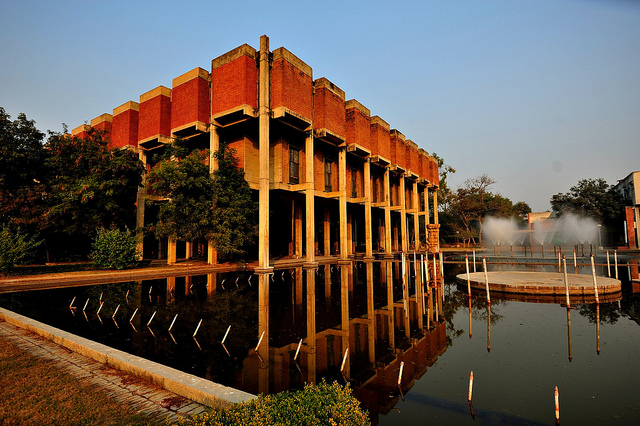
\includegraphics[width=0.6\textwidth]{images/lib.jpg}
\end{center}

\section{Welcome}

\vspace{-1em}

Welcome to the international symposium "Molecular Simulations of Complex Fluids and Interfaces", hosted at IIT Kanpur.

The behaviour of interfaces plays an important role in several industrial and natural processes. Molecular simulations can reveal microscopic insights into the structure and properties of solid-liquid interfaces. This meeting aims to provide a forum for exchanging ideas and sharing recent scientific advances from several perspectives. It is hoped that the current state of simulation methodologies will be established, paving the way for the future development of computational tools and research.

\vspace{-2em}

\section{Topics}

\vspace{-1em}

\begin{itemize}
  \itemsep-1em 
  \item Molecular Simulations: New Methodologies and Applications
  \item Advances in Coarse-Graining and Challenges
  \item Soft Matter Simulations
  \item Confined Fluids
  \item Wetting and Interfacial Phenomena
  \item Biomolecular Simulations
  \item Specific Systems and Models
\end{itemize}

% \pagebreak

% The following topics will be covered in the planned talks and lectures.



% \section{Organizing committee}
% \begin{center}
% \begin{tabular}{lll}
% Gloria Cecchini & Marco Faggian &  Aleksandra Pidde \\
% Rok Cestnik & R. Janis Goldschmidt &  Bastian Pietras\\
%  Pau Clusella  & Marc Grau Leguia & Eero Satuvuori \\
%  Nicolás Deschle & Maxime Lucas   &  Çağdaş Topçu \\
% Federico Devalle  & Irene Malvestio  & Clément Zankoc 
% \end{tabular}
% \end{center}

% TIMETABLE 
%---------------------------------------------------------------------
\chapter{Timetable}

KL: Keynote Lecture, IS: Invited Speaker, ST: Sponsored Talk.
% Custom commands used here can be found at the end of the preamble_booklet.tex file

\section{February 21, Friday}
\begin{center}
	\filbreak
\begin{longtable}{|C{0.15\linewidth}| C{0.04\linewidth}|  C{0.3\linewidth} C{0.0\linewidth} C{0.4\linewidth}|}\hline	
	\tablebreak{15:00--16:00}{Registration}
	\tablebreak{16:00--16:15}{Inauguration Ceremony}
	\KL{16:15--17:15}{Florian Müller-Plathe}{}{\small{Technische Universität Darmstadt}}{Wetting, Drying, Adhesion}
	\IS{17:15--17:40}{Neelanjana Sengupta}{}{IISER Kolkata}{Modulating Self-Assembled Amyloidogenic States via Solvent and Temperature: Insights from Computer Simulations}
	\IS{17:40--18:05}{Harshwardhan Katkar}{}{IIT Kanpur}{Multiscale Modeling of Actin Filaments}
	\IS{18:05--18:30}{Manjesh K. Singh}{}{IIT Kanpur}{Rheology of Nonequilibrium Polymer Melts}
	\eventtype{19:00--21:30}{Reception Dinner}
\end{longtable}
\end{center}

\newpage
\section{February 22, Saturday}
\begin{center}
	\begin{longtable}{|C{0.15\linewidth}| C{0.04\linewidth}|  C{0.3\linewidth} C{0.0\linewidth} C{0.4\linewidth}|}\hline	
		\KL{9:30--10:30}{Edward Maginn}{}{University of Notre Dame}{Computational Design of New Materials for Separations and Energy Storage}
		\tablebreak{10:30--11:00}{Tea Break}
		\IS{11:00--11:25}{Beena Rai}{}{Tata Research Development and Design Center}{Skin Lipids and their Interfaces: A Computational Approach towards Mimicking Skin Barrier Function}
		\IS{11:25--11:50}{Sudip Roy}{}{National Chemical Lab, India}{Bridging Scales for Simulation of Lipids}
		\IS{11:50--12:15}{Swati Bhattacharya}{}{IIT Bombay}{Molecular Dynamics Investigations of anti HIV-1 protein SAMHD1}
		\IS{12:15--12:40}{R. Sankararamakrishnan}{}{IIT Kanpur}{TBA}
		\tablebreak{12:40--14:00}{Lunch Break}
		\KL{14:00--15:00}{Balasubramanian Sundaram}{}{JNCASR}{Modelling Supramolecular Polymers}
		\IS{15:00--15:25}{Divya Nayar}{}{IIT Kharagpur}{Microscopic View of the Crowding Effects on Hydrophobic Collapse}
		\IS{15:25--15:50}{Nisanth N. Nair}{}{IIT Kanpur}{Exploration of High Dimensional Free Energy Landscapes of Chemical Reactions}
		\tablebreak{15:50--16:20}{Tea Break}
		\IS{16:20--16:45}{Rajat Srivastava}{}{Politecnico di Torino}{Thermo-Physical Properties of Graphene Reinforced Thermoplastics: A Coarse-Grained Modelling Approach}
		\IS{16:45--17:10}{Tamal Banerjee}{}{IIT Guwahati}{Reactive Force Field Simulations on the Degradation of Quinoline}
		\ST{17:10--17:30}{Ashwini Kumar}{}{NEC Corp.}{Vector Computing- Simulation and A.I.}
		\eventtype{17:30--18:55}{Poster Presentation Session}
		\eventtype{18:55--19:00}{Announcement of Springer Best Poster Awards}
	\end{longtable}
\end{center}

% \newpage
% \vfill

% \vspace{-10em}

\section{February 23, Sunday}
\vspace{-1em}
\begin{center}
	\begin{longtable}{|C{0.15\linewidth}| C{0.04\linewidth}|  C{0.3\linewidth} C{0.0\linewidth} C{0.4\linewidth}|}\hline	
		\KL{9:30 --10:30}{David A. Kofke}{}{SUNY, Buffalo}{'Mapped Averaging’ Method for deriving Ensemble Averages: Application to Crystals}
		\tablebreak{10:30--11:00}{Tea Break}
		\IS{11:00--11:25}{Shantanu Maheshwari}{}{Shell Technology}{Nucleation and Growth of a Nanobubble on Rough Surfaces}
		\IS{11:25--11:50}{Kaustubh Rane}{}{IIT Gandhinagar}{The Role of Solid-Liquid Interfacial Fluctuations in the Spontaneous Motion of Droplets}
		\IS{11:50--12:15}{Sandip Khan}{}{IIT Patna}{The Wetting Behavior of Imidazolium Based Ionic Liquids using Molecular Dynamics Simulation}
		\IS{12:15--12:40}{Jhumpa Adhikari}{}{IIT Bombay}{Phase Equilibria of Binary Mixtures of Triangle-Well Fluids : Bulk vs Confined Systems}		
		\tablebreak{12:40--14:00}{Lunch Break}
		\IS{14:00--14:25}{Sudeep Punnathanam}{}{IISC Bangalore}{Computing Solid-Liquid Interfacial Free Energy via Thermodynamic Integration}
		\IS{14:25--14:50}{Subir K. Das}{}{JNCASR}{Kinetics of Clustering in an Assembly of Vicsek-Like Active Particles}
		\IS{14:50--15:15}{Tarak Patra}{}{IIT Madras}{Correlation between Glass Formation and Ion Conductivity in Polymeric Ionic Liquids}
		\IS{15:15--15:40}{Prateek Kumar Jha}{}{IIT Roorkee}{Multiscale Modeling Approaches in Excipient Design for Oral Drug Delivery}
		\tablebreak{15:40--16:10}{Tea Break}
		\IS{16:10--16:35}{Sk. Musharaf Ali}{}{BARC, Mumbai}{Microscopic Assessment of Liquid-Liquid Extraction System in Bulk and at the Interface}
		\IS{16:35--17:00}{Vishwanath Dalvi}{}{ICT, Mumbai}{Study of Water Extraction by Phosphate Ligands by Experiments and Molecular Simulations}
		\IS{17:00--17:25}{Rajat Desikan}{}{Invictus Oncology Pvt. Ltd.}{Accurate Computational Calorimetry of Lipid Membranes by void-induced Melting}
		\eventtype{17:25--17:35}{Springer Poster Awardee Talk-1}
		\eventtype{17:35--17:45}{Springer Poster Awardee Talk-2}
		\eventtype{17:45--18:00}{Vote of Thanks}
		\eventtype{19:00--21:30}{Symposium Dinner}
	\end{longtable}
\end{center}


% TALKS 
%---------------------------------------------------------------------
\chapter{List of Abstracts -- Talks}

\section{February 21, Friday}

% Definitions of custom environment used here can be found in preamble_booklet.tex file

% The following input commands automatically select the right version 
% (print or online) version of the abstract's .tex
% \type is defined in preamble_booklet.tex and equals:
% 'o' (online) or 'p' (print)

\input{abstracts/tex/t\type_florian} % KL
\input{abstracts/tex/t\type_neelanjana} % Neelanjana Sengupta
\input{abstracts/tex/t\type_katkar} % Harshwardhan Katkar
\input{abstracts/tex/t\type_manjesh} % Manjesh K. Singh

% \vspace{30em}
\vfill

\section{February 22, Saturday}

\input{abstracts/tex/t\type_maginn} % KL Edward Maginn
\input{abstracts/tex/t\type_beena} % Beena Rai
\input{abstracts/tex/t\type_sudip} % Sudip Roy
\input{abstracts/tex/t\type_swati} % Swati Bhattacharya
\input{abstracts/tex/t\type_ramasubbu} % R. Sankararamakrishnan
\input{abstracts/tex/t\type_bala} % KL Balasubramanian Sundaram
\input{abstracts/tex/t\type_divya} % Divya Nayar
\input{abstracts/tex/t\type_nair} % Nisanth Nair
\input{abstracts/tex/t\type_rajat} % Rajat Srivastava
\input{abstracts/tex/t\type_tamal} % Tamal Banerjee
\input{abstracts/tex/t\type_nec} % Sponsored talk by NEC (Ashwini Kumar)

\vfill

\section{February 23, Sunday}

\input{abstracts/tex/t\type_kofke} % KL David Kofke
\input{abstracts/tex/t\type_shantanu} % Shantanu Maheshwari
\input{abstracts/tex/t\type_rane} % Kaustubha Rane
\input{abstracts/tex/t\type_sandip}
\input{abstracts/tex/t\type_jumpa}
\input{abstracts/tex/t\type_punna}
\input{abstracts/tex/t\type_subir} % Subir K. Das
\input{abstracts/tex/t\type_tarak} % Tarak Patra
\input{abstracts/tex/t\type_prateek} % Prateek Kumar Jha
\input{abstracts/tex/t\type_musharaf}
\input{abstracts/tex/t\type_vishwa} % Vishwanath H. Dalvi
\input{abstracts/tex/t\type_desikan} % Rajat Desikan


% POSTERS
%------------------------------------------------------------------
\chapter{List of Posters} 

% \vspace{-2.5em}

% \section{February 22, Saturday}

\input{abstracts/tex/p\type_nikhil-avula} % Nikhil V. S. Avula
\input{abstracts/tex/p\type_dueby} % Shivam Dueby
\input{abstracts/tex/p\type_nirali-desai} % Nirali Desai
\input{abstracts/tex/p\type_sonali-gore} % Sonali Gore
\input{abstracts/tex/p\type_arya} % Arya Das
\input{abstracts/tex/p\type_vikas-dubey} % Vikas Dubey
\input{abstracts/tex/p\type_hrushikesh} % Hrushikesh M. Gade
\input{abstracts/tex/p\type_omkar-singh} % Omkar Singh
\input{abstracts/tex/p\type_sagar-kamble} % Sagar Kamble
\input{abstracts/tex/p\type_projesh-roy} % Projesh K. Roy
\input{abstracts/tex/p\type_bharti} % Bharti
\input{abstracts/tex/p\type_shivanand-veesam} % Shivanand Kumar Veesam
\input{abstracts/tex/p\type_ravi-reddy} % Ravi Kumar Reddy
\input{abstracts/tex/p\type_krishna-jaiswal} % Krishna Jaiswal
\input{abstracts/tex/p\type_shubhandra} % Shubhandra Tripathi
\input{abstracts/tex/p\type_sanchari} % Sanchari Bhattacharjee
\input{abstracts/tex/p\type_nandlal} % Nandlal Pingua

% LIST OF PARTICIPANTS
%------------------------------------------------------------------
% \chapter{List of Posters} %List of Participants
 
% % The array below was automatically created from a spreadsheet with 'calc2latex'

% \begin{center}
% \rowcolors{1}{gray!25}{white}
% \begin{longtable}{p{0.4\linewidth} p{0.4\linewidth} }
% \hline
% 		John1 Doe1 & Barcelona, Spain \\ \hline
% 		John2 Doe2 & Barcelona, Spain \\ \hline
% 		John3 Doe3 & Barcelona, Spain \\ \hline
% 		John4 Doe4 & Barcelona, Spain \\ \hline
% 		John5 Doe5 & Barcelona, Spain \\ \hline
% 		John6 Doe6 & Barcelona, Spain \\ \hline
% 		John7 Doe7 & Barcelona, Spain \\ \hline
% 		John8 Doe8 & Barcelona, Spain \\ \hline
% 		John9 Doe9 & Barcelona, Spain \\ \hline
% 		John10 Doe10 & Barcelona, Spain \\ \hline
% 		John11 Doe11 & Barcelona, Spain \\ \hline
% 		John12 Doe12 & Barcelona, Spain \\ \hline
% 		John13 Doe13 & Barcelona, Spain \\ \hline
% 		John14 Doe14 & Barcelona, Spain \\ \hline
% 		John15 Doe15 & Barcelona, Spain \\ \hline
% 		John16 Doe16 & Barcelona, Spain \\ \hline
% 		John17 Doe17 & Barcelona, Spain \\ \hline
% 		John18 Doe18 & Barcelona, Spain \\ \hline
% 		John19 Doe19 & Barcelona, Spain \\ \hline
% 		John20 Doe20 & Barcelona, Spain \\ \hline
% 		John21 Doe21 & Barcelona, Spain \\ \hline
% 		John22 Doe22 & Barcelona, Spain \\ \hline
% 		John23 Doe23 & Barcelona, Spain \\ \hline
% 		John24 Doe24 & Barcelona, Spain \\ \hline
% 		John25 Doe25 & Barcelona, Spain \\ \hline
% 		John26 Doe26 & Barcelona, Spain \\ \hline
% 		John27 Doe27 & Barcelona, Spain \\ \hline
% 		John28 Doe28 & Barcelona, Spain \\ \hline
% 		John29 Doe29 & Barcelona, Spain \\ \hline
% \end{longtable}
% \end{center}

% Please add the following required packages to your document preamble:
% \usepackage{booktabs}
\begin{center}
\begin{longtable}{@{}ll@{}}
\toprule
\multicolumn{1}{c}{\textbf{Presenter}}                              & \multicolumn{1}{c}{\textbf{Poster Title}}                                                                                                                                                                              \\ \midrule
Shubham Tiwari                                                      & \begin{tabular}[c]{@{}l@{}}Insight to the Mechanism of Nanoparticle Induced\\ Suppression of Detergency: Theory and Simulations\end{tabular}                                                                           \\
Hrushikesh M. Gade                                                  & \begin{tabular}[c]{@{}l@{}}Water-mediated curvature change in graphene by\\ single-walled carbon nanotube: A molecular dynamics\\ study\end{tabular}                                                                   \\
\begin{tabular}[c]{@{}l@{}}Avula Venkata Siva\\ Nikhil\end{tabular} & Atomistic Modeling of Binary Ionic Liquid Mixtures                                                                                                                                                                     \\
Prosun Halder                                                       & \begin{tabular}[c]{@{}l@{}}High Throughput Screening of Hypothetical Metal\\ Organic Frameworks for Ethane-Ethylene Separation\end{tabular}                                                                            \\
Sonali Gore                                                         & \begin{tabular}[c]{@{}l@{}}Tuning the Adsorption Behaviour of the Material at the\\ Molecular Scale to Get the Desired Macroscopic\\ Behaviour by Using Statistical Mechanics and\\ Molecular Simulations\end{tabular} \\
Shakkira Erimban                                                    & \begin{tabular}[c]{@{}l@{}}Cold Adaptation of Cell Membrane of a\\ Psychrotolerant Bacteria: Investigation using\\ Molecular Dynamics Simulation\end{tabular}                                                          \\
Vikas Dubey                                                         & \begin{tabular}[c]{@{}l@{}}Mechanism of Hydroxide Ion Transfer through Anion\\ Exchange Membrane in Anion Exchange Membrane\\ Fuel Cell: Investigation using Molecular Dynamics\\ Simulation\end{tabular}              \\
Nirali Dhiren Desai                                                 & \begin{tabular}[c]{@{}l@{}}New Age Antimicrobial Peptides: Revealing Mode of\\ Actions of Multifunctional AMPs Using Molecular\\ Dynamics Study\end{tabular}                                                           \\
Shivam Dubey                                                        & \begin{tabular}[c]{@{}l@{}}Role of Translational Jump-diffusion in the\\ Breakdown of the Stokes-Einstein relation in\\ Supercooled Water and its Binary Mixture with\\ Glycerol\end{tabular}                          \\
Omkar Singh                                                         & \begin{tabular}[c]{@{}l@{}}Characterization of Biological Water at Interface of\\ Antimicrobial Peptide in Presence of Salts Solution\end{tabular}                                                                     \\
Arya Das                                                            & \begin{tabular}[c]{@{}l@{}}Molecular Dynamics Simulations on Interfacial\\ Structure in Presence of Third Component\end{tabular}                                                                                       \\
Projesh Kumar Roy                                                   & \begin{tabular}[c]{@{}l@{}}Microscopic structure and CO2 adsorption properties\\ of 6FDA/BPDA-DAM polymeric membrane\end{tabular}                                                                                      \\
\begin{tabular}[c]{@{}l@{}}Gauri Tekbahadur\\ Thapa\end{tabular}    & \begin{tabular}[c]{@{}l@{}}Molecular Dynamics Simulation of Anti-HIV Protein\\ SAMHD1\end{tabular}                                                                                                                     \\
\toprule
\\
\midrule
{\textbf{Presenter}}                              & \multicolumn{1}{c}{\textbf{Poster Title}}                                                                                                                                                                              \\ \midrule
Bharti                                                              & \begin{tabular}[c]{@{}l@{}}Melting in Two-Dimensional Gay-Berne Liquid\\ Crystals\end{tabular}                                                                                                                         \\
Manjinder Singh                                                     & \begin{tabular}[c]{@{}l@{}}A Comparative Study of Tackifying Monomers to\\ Develop Bio-Based Pressure-Sensitive Adhesive: A\\ Computational Approach\end{tabular}                                                      \\
Ravi Kumar Reddy A                                                  & \begin{tabular}[c]{@{}l@{}}Uncovering the Molecular Mechanism of Solvent\\ Induced Polymorphism in Crystal Nucleation from\\ Solution\end{tabular}                                                                     \\
Jyoti Kuntail                                                       & \begin{tabular}[c]{@{}l@{}}Understanding the Adsorption Mechanism of\\ Arsenous acid on Magnetite (311) Surface through\\ Molecular Dynamics simulations\end{tabular}                                                  \\
Rajneesh Kashyap                                                    & \begin{tabular}[c]{@{}l@{}}Oil Detachment from Rock Surface using\\ Nanoparticles, Surfactant and low salinity brine: A\\ Molecular Dynamic Study\end{tabular}                                                         \\
\begin{tabular}[c]{@{}l@{}}Shivanand Kumar\\ Veesam\end{tabular}    & \begin{tabular}[c]{@{}l@{}}Molecular Modelling of Phase Equilibrium of Gas\\ Hydrates\end{tabular}                                                                                                                     \\
Jagroop Kaur                                                        & \begin{tabular}[c]{@{}l@{}}Temperature Dependent Interaction of Soft Repulsive\\ Wall with the Thermotropic Liquid Crystals\end{tabular}                                                                               \\
Krishna Jaiswal                                                     & \begin{tabular}[c]{@{}l@{}}A Functional Force Field Model for Water based on\\ Gaussian Charges\end{tabular}                                                                                                           \\
Sanchari Bhattacharjee                                              & \begin{tabular}[c]{@{}l@{}}Effect of Alkyl chain on The Wetting Behaviour of\\ Aqueous Ionic Liquids: A Molecular Dynamics Study\end{tabular}                                                                          \\
Shubhandra Tripathi                                                 & \begin{tabular}[c]{@{}l@{}}A Temperature Accelerated Sliced Sampling study of\\ Drug Binding/Unbinding\end{tabular}                                                                                                    \\
Sagar Dinkar Kamble                                                 & \begin{tabular}[c]{@{}l@{}}Investigation of Cholesterol Influence in Fluid Phase\\ and Gel Phase Lipid Bilayers by Coarse-grained\\ Molecular Dynamic Simulation\end{tabular}                                          \\
Showkat Mir                                                         & \begin{tabular}[c]{@{}l@{}}Electronic Properties of High $CO_2$ Capture Ability of\\ Two-Dimensional Metal Nitrides (XN; X=Al, Ga, In): A\\ Computational Study\end{tabular}                                           \\
Amrita Goswami                                                      & \begin{tabular}[c]{@{}l@{}}Formulation and Implementation of General\\ Topological Network Criteria for Exploring the\\ Structures of Confined Ice\end{tabular}                                                        \\ \bottomrule
\end{longtable}
\end{center}
 
% USEFUL INFO
%------------------------------------------------------------------
% \chapter{Useful Information}

% \input{useful_info}

% SPONSORS
%------------------------------------------------------------------
\chapter{Sponsors}

% \begin{center}
% The AMCOS conference is part of the COSMOS project, funded by the European Union’s Horizon 2020 research and innovation programme under the Marie Sk\l{}odowska-Curie grant agreement No 642563.
% \end{center}

% \vfill

% \section{Sponsors}

% \begin{center}
% \includegraphics[width=0.5\textwidth]{images/logos/Partnerlogos/LancasterHelium.jpg}
% \includegraphics[width=0.5\textwidth]{images/logos/Partnerlogos/springer.pdf}
% \end{center}

\vfill

\begin{center}

\includegraphics[width=\textwidth]{images/logos/sponsors2.png}

\vfill


\includegraphics[width=\textwidth]{images/logos/diamondJubilee.png}
\end{center}

\newpage

% BACK PAGE
%-----------------------------------------------------------------

\pagecolor{myblue}
\thispagestyle{empty}
\mbox{}

\end{document}
